\usetikzlibrary{positioning,fit,calc} % used for the efficient working of the positioning system  
\tikzset{block/.style={draw, thick, text width=3cm, minimum height=1.5cm, align=center},   
line/.style={-latex}
}

Here's a simplified TikZ representation of the top-level structure:

\begin{center}
  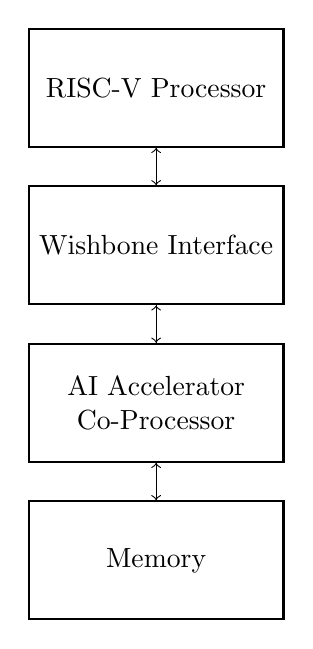
\begin{tikzpicture}[node distance=2cm, every node/.style={align=center}]
    % Nodes
    \node [block] (riscv) {RISC-V Processor};
    \node [block, below of=riscv] (wishbone) {Wishbone Interface};
    \node [block, below of=wishbone] (coprocessor) {AI Accelerator Co-Processor};
    \node [block, below of=coprocessor] (memory) {Memory};
    % Arrows
    \draw [->] (riscv) -- (wishbone);
    \draw [->] (wishbone) -- (coprocessor);
    \draw [->] (coprocessor) -- (memory);
    \draw [->] (memory) -- (coprocessor);
    \draw [->] (coprocessor) -- (wishbone);
    \draw [->] (wishbone) -- (riscv);
  \end{tikzpicture}
\end{center}

In this diagram, the RISC-V processor is at the top, followed by the Wishbone interface, which serves as the communication interface between the RISC-V processor and the AI accelerator co-processor.
The AI accelerator co-processor contains the AI accelerator ASIC, which implements the tensor operations and other mathematical operations you mentioned earlier.
The memory block represents the shared memory used for data exchange between the RISC-V processor and the co-processor.
